% ----------------------------------------------------------
\chapter{TENSORES} \label{Tensor}
% ----------------------------------------------------------

%\lipsum[50]

Na Física e nas Engenharias as grandezas podem ser classificadas em três grandes grupos:

\begin{enumerate}
	
	\item Grandezas escalares: são aquelas que necessitam de somente uma informação para classificá-las. Como exemplos destas grandezas tem-se a temperatura, comprimento, massa, tempo, volume, energia, entre outros.
	\item Grandezas vetoriais: são as que necessitam de três informações para caracterizá-las (módulo, direção e sentido). Como exemplos destas grandezas pode-se destacar o deslocamento, a força, o fluxo, a corrente elétrica e a aceleração.
	\item Grandezas Tensoriais: são aquelas que para serem bem representadas necessitam de, pelo menos, nove informações. Destacam-se como exemplos o tensor de tensão, o tensor de deformação, o tensor inercial e as rotações. 
\end{enumerate}

A transformação linear que tem a capacidade de transformar um dado vetor $ \vec{a} $ em um outro vetor $ \vec{b} $, ou seja,
\begin{equation}
	\vec{a} = \textbf{T} \vec{b}
\end{equation}
é chamada de tensor de segunda ordem ou simplesmente de tensor, cuja notação é $ \textbf{T} $. Assim, $ \textbf{T} $ é uma transformação linear, pois
\begin{equation}
	\textbf{T} ( \alpha \vec{a} + \beta \vec{b}) = \alpha \textbf{T}( \vec{a}) + \beta \textbf{T} ( \vec{b}).
\end{equation}

Para um conjunto de vetores unitários $ e_{1}, e_{2}, e_{3} $, na direção das componentes de um sistema de coordenadas retangulares, suas transformações podem ser escritas na forma
\begin{equation}
	\textbf{T} e_{1} = \textbf{T} \left[ 
	\begin{array}{c}
		1\\
		0\\
		0\\
	\end{array}
	\right] = \textbf{T} (1 e_{1} + 0 e_{2} + 0 e_{3}) 
\end{equation} 
ou
\begin{equation} \label{TFe1}
	\textbf{T} e_{1} = T_{11} e_{1} + T_{21} e_{2} + T_{31} e_{3},
\end{equation}
\begin{equation} \label{TFe2}
	\textbf{T} e_{2} = T_{12} e_{1} + T_{22} e_{2} + T_{32} e_{3},
\end{equation}
\begin{equation}\label{TFe3}
	\textbf{T} e_{3} = T_{13} e_{1} + T_{23} e_{2} + T_{33} e_{3}.
\end{equation}

Utilizando a notação indicial esta transformação pode ser generalizada como
\begin{equation} \label{indicialT}
	\textbf{T} e_{i} = T_{ji} e_{j}.
\end{equation}

Considerando as transformações apresentadas em (\ref{TFe1}), (\ref{TFe2}) e (\ref{TFe3}), o tensor \textbf{T} pode ser representado matricialmente da seguinte forma
\begin{equation} \label{matrizT}
	\textbf{T} = [T] =  \left[ 
	\begin{array}{ccc}
		T_{11} & T_{12} & T_{13} \\
		T_{21} & T_{22} & T_{23} \\
		T_{31} & T_{32} & T_{33} \\
	\end{array}
	\right].  
\end{equation} 

Assim como na transformação linear, os tensores também apresentam algumas propriedades. São elas:
\begin{enumerate}
	\item[a)] A soma entre dois tensores \textbf{T} e \textbf{S}
	\begin{equation}
		( \textbf{T} + \textbf{S}) \vec{a} = \textbf{T} \vec{a} + \textbf{S} \vec{a}, 
	\end{equation}
	que, em notação indicial, é escrito como
	\begin{equation}
		W_{ij} = T_{ij} + S_{ij}.
	\end{equation}
	\item[b)] O produto de dois tensores, caracteriza-se por
	\begin{equation}
		( \textbf{T} \textbf{S}) \vec{a} = \textbf{T} ( \textbf{S} \vec{a})
	\end{equation}
	ou
	\begin{equation}
		(TS)_{ij} = T_{im} S_{mj}.
	\end{equation}
	\item[c)] Transposição de um tensor $( \textbf{T} ^{T})$
	\begin{equation}
		\vec{a} \cdot \textbf{T} \vec{b} = \vec{b} \cdot \textbf{T} ^{T} \vec{a}.
	\end{equation}
	\item[d)] O traço de um tensor \textbf{T} é representado em notação indicial por
	\begin{equation}
		tr \textbf{T} = T_{ij} \delta _{ij},
	\end{equation}
	onde
	\begin{equation}
		\delta _{ij} = \left\{
		\begin{array}{rcl}
			1 & se & i = j\\
			0 & se & i \neq j
		\end{array} \right.,
	\end{equation}
	é o delta de Kronecker.
	\item[e)] Um tensor \textbf{T} pode ser decomposto em uma parte simétrica, $ \textbf{T} ^{S} $, e uma parte antissimétrica, $ \textbf{T} ^{A} $, ou seja,
	\begin{equation}
		\textbf{T} = \textbf{T} ^{S} + \textbf{T} ^{A},
	\end{equation}
	\begin{equation}
		\textbf{T} ^{S} = \dfrac{ \textbf{T} + \textbf{T} ^{T}}{2},
	\end{equation}
	e
	\begin{equation}
		\textbf{T} ^{A} = \dfrac{ \textbf{T} - \textbf{T} ^{T}}{2}.
	\end{equation}
\end{enumerate}

No cálculo tensorial, se $ \textbf{T} = \textbf{T} (t) $ for um tensor de segunda ordem dependente do tempo, então
\begin{equation}
	\dfrac{d \textbf{T}}{dt} = \lim_{ \Delta t \to 0} \dfrac{ \textbf{T} ( t+ \Delta t) - \textbf{T} (t)}{ \Delta (t)}
\end{equation}
e
\begin{equation}
	\dfrac{d}{dt} [ \textbf{T} + \textbf{S}] = \dfrac{d \textbf{T}}{dt} + \dfrac{d \textbf{S}}{dt}.
\end{equation}

Se $ \alpha(t)$ for um escalar dependente do tempo, então
\begin{equation}
	\dfrac{d}{dt}  [ \alpha(t) \textbf{T}] = \dfrac{d \alpha(t)}{dt} \textbf{T} + \alpha(t) \dfrac{d \textbf{T}}{dt}.
\end{equation}

Se $ [ \textbf{T} \textbf{S}]$ for o produto entre dois tensores, então
\begin{equation}
	\dfrac{d}{dt} [ \textbf{T} \textbf{S}] = \dfrac{d \textbf{T}}{dt} \textbf{S} + \textbf{T} \dfrac{d \textbf{S}}{dt}. 
\end{equation}

Se $ [ \textbf{T} \vec{a}]$ representa a transformação de um vetor $ \vec{a}$, então
\begin{equation}
	\dfrac{d}{dt} [ \textbf{T} \vec{a}] = \dfrac{d \textbf{T}}{dt} \vec{a} + \textbf{T} \dfrac{d \vec{a}}{dt}.
\end{equation}

Se $[ \textbf{T} ^{T}]$ representar um tensor transposto, então
\begin{equation}
	\dfrac{d}{dt} [ \textbf{T} ^{T}] =
	\left[
	\begin{array}{c}
		\dfrac{d \textbf{T}}{dt}\\
	\end{array} \right] ^{T} .
\end{equation}

Para um campo vetorial o divergente de um vetor velocidade $ \vec{v}$ é calculado, segundo \citeonline{Malvern}, por
\begin{equation}
	\mbox{div} \vec{v} = tr [ { \nabla} \vec{v}] = { \nabla} \cdot \vec{v}
\end{equation} 
onde $ { \nabla} $ é o operador gradiente. Assim, tem-se que, em relação às suas componentes,
\begin{equation}
	\mbox{div} \vec{v} = \dfrac{ \partial v_{1}}{ \partial x_{1}} + \dfrac{ \partial v_{2}}{ \partial x_{2}} +\dfrac{ \partial v_{3}}{ \partial x_{3}}.
\end{equation}

Para um campo tensorial, o divergente deste campo é calculado pela equação
\begin{equation}
	(\mbox{div} \textbf{T}) \cdot \vec{a} = \mbox{div} ( \textbf{T} ^{T} \vec{a}) - tr ( \textbf{T} ^{T} ( { \nabla} \vec{a}))
\end{equation}
ou, em notação indicial,
\begin{equation}
	\mbox{div} \textbf{T} = \dfrac{ \partial T_{im}}{ \partial x_{m}} \vec{e} _{i}.
\end{equation}

Em certos problemas da engenharia que envolvem pequenos deslocamentos faz-se necessário conhecer e descrever suas deformações. Quando estas deformações são muito pequenas dá-se o nome de deformações infinitesimais \cite{Lai}.

Considerando a Figura \ref{fig:campodeform}, em um dado instante $ t_{0} $, os pontos $ P(t_{0}) $ e $ Q(t_{0}) $ apresentam um vetor distância $ \vec{dX} $. Para este instante $ t_{0} $ diz-se que os pontos estão na configuração $ B_{0} $. Após um certo instante de tempo $ t $ ocorre o deslocamento dos pontos $ P $ e $ Q $, sendo chamados agora de $ P(t) $, $ Q(t) $  e a nova configuração de $ B_{t} $, o que infere uma mudança em $  \vec{dX} $ passando a ser chamado de $  \vec{dx} $. Esta variação de deslocamento, por ser infinitesimal, pode ser considerada como um filamento. Logo, o filamento  $  \vec{dx} $ é dado por:
\begin{equation} \label{filamento}
	\vec{dx} = \vec{dX} + ( { \nabla} \vec{u}) \vec{dX},
\end{equation}
onde
\begin{equation}
	{ \nabla} \vec{u} = \left[
	\begin{array}{ccc}
		\dfrac{ \partial u_{1}}{ \partial x_{1}} & \dfrac{ \partial u_{1}}{ \partial x_{2}} & \dfrac{ \partial u_{1}}{ \partial x_{3}}\\
		
		\dfrac{ \partial u_{2}}{ \partial x_{1}} & \dfrac{ \partial u_{2}}{ \partial x_{2}} & \dfrac{ \partial u_{3}}{ \partial x_{3}}\\
		
		\dfrac{ \partial u_{3}}{ \partial x_{1}} & \dfrac{ \partial u_{3}}{ \partial x_{2}} & \dfrac{ \partial u_{3}}{ \partial x_{3}}\
	\end{array} \right],
\end{equation}
é o tensor gradiente de deslocamentos.

\begin{figure}[H]
	\centering
	\includegraphics[scale=1]{figuras/campo_de_deformacao.jpg}
	\caption{\textsc{Deformação infinitesimal}}
	\vspace{-0.1cm}
	\legend{FONTE: \citeonline{Lai}}
	\label{fig:campodeform}
\end{figure}

%\begin{figure}
%\caption{DEFORMAÇÃO INFINITESIMAL}
%\small{Fonte: LAI, 2010}
%\label{fig:campodeform}
%\centering
%\includegraphics[scale=1]{campo_de_deformacao.jpg}
%\end{figure}	


O filamento $ \vec{dx} $ na equação (\ref{filamento}) pode ser escrita como 
\begin{equation}
	\vec{dx} = [ \textbf{I} + ( { \nabla} \vec{u})] \vec{dX} 
\end{equation}
onde \textbf{I} é o  tensor identidade. Logo, 
\begin{equation} \label{filamento_dx}
	\vec{dx} = \textbf{F} \vec{dX},
\end{equation}
sendo
\begin{equation} \label{tensordeform}
	\textbf{F} = \textbf{I} + ( { \nabla}  \vec{u}).
\end{equation}
Mas
\begin{equation}
	\textbf{F} ^T \cdot \textbf{F} = ( \textbf{I} + { \nabla}  \vec{u}) ^T \cdot ( \textbf{I} + { \nabla}  \vec{u}) 
\end{equation}
o que resulta em
\begin{equation} \label{FtranspF}
	\textbf{F} ^T \cdot \textbf{F} = \textbf{I} + ( { \nabla}  \vec{u}) + ( { \nabla}  \vec{u}) ^T +  ( { \nabla}  \vec{u}) ^T ( { \nabla}  \vec{u}).
\end{equation}

Considerando que a magnitude do vetor $  \vec{u} $ é muito pequena, $  \Vert \vec{u} \Vert < < 1  $ , então       
\begin{equation}
	( { \nabla}  \vec{u}) ^T ( { \nabla}  \vec{u}) \approx 0,
\end{equation}
que, substituindo na equação (\ref{FtranspF}), resulta
\begin{equation}
	\textbf{F} ^T \cdot \textbf{F} = \textbf{I} + ( { \nabla}  \vec{u}) + ( { \nabla}  \vec{u}) ^T .
\end{equation}

Assumindo
\begin{equation}
	\textbf{E} = \dfrac{ ( { \nabla}  \vec{u}) + ( { \nabla}  \vec{u}) ^T}{2}
\end{equation}
como sendo um tensor simétrico de $ ( { \nabla}  \vec{u})   $, então
\begin{equation}
	\textbf{F} ^T \cdot \textbf{F} = \textbf{I} + 2 \textbf{E},
\end{equation}      
sendo \textbf{E} chamado de tensor de deformações infinitesimais.
Assim com foi feito nas equações (\ref{indicialT}) e (\ref{matrizT}), o tensor \textbf{E} também pode ser escrito na forma matricial
\begin{equation}
	[E] =  \left[ 
	\begin{array}{ccc}
		E_{11} & E_{12} & E_{13} \\
		E_{21} & E_{22} & E_{23} \\
		E_{31} & E_{32} & E_{33} \\
	\end{array}
	\right] _{X_{1} X_{2} X_{3}}.  
\end{equation}

No entanto, se as deformações ocorrerem somente nas direções principais, ou seja, nas direções dos autovetores  do tensor \textbf{E}, então
\begin{equation}
	[E] =  \left[ 
	\begin{array}{ccc}
		E_{1} & 0 & 0 \\
		0 & E_{2} & 0 \\
		0 & 0 & E_{3} \\
	\end{array}
	\right]  
\end{equation}
e, neste caso, haverá na transformação uma preservação dos ângulos, sendo chamada de uma transformação pura \cite{Lai}.

\begin{figure}[H]
	\centering
	\includegraphics[scale=1]{figuras/deformacoes.jpg}
	\caption{\textsc{Campo de deslocamentos}}
	\vspace{-0.1cm}
	\legend{FONTE: \citeonline{Lai}}
	\label{fig:campodesl}
\end{figure}

%\begin{figure}
%\caption{CAMPO DE DESLOCAMENTOS}
%\label{fig:campodesl}
%\centering
%\includegraphics[scale=1]{deformacoes.jpg}
%\end{figure}


A Figura \ref{fig:campodesl} apresenta o deslocamento de um dado corpo rígido no instante $ t_{0} $ e após um instante $ t $. Nota-se, em relação à sua configuração inicial, que este corpo sofreu dois movimentos, sendo um de rotação e o outro de deformação. Assim, sejam \textbf{U} e \textbf{V} tensores simétricos e \textbf{R} um tensor ortogonal próprio. Tomando como base a equação (\ref{tensordeform}), o tensor \textbf{F} pode ser escrito como
\begin{equation} \label{Caucy_dir}
	\textbf{F} = \textbf{R} \textbf{U}
\end{equation}    
e
\begin{equation} \label{Caucy_esq}
	\textbf{F} = \textbf{V} \textbf{R}.
\end{equation}


%-----------------------------------------------------
%para trabalhar com referencias para equações
%incluir o label com um nome para a equacao e referenciar no texto com ~\ref{label} 
%\begin{equation}\label{nome}
%\textbf{F} = \textbf{V} \textbf{R}.
%\end{equation}
%-----------------------------------------------------

As equações (\ref{Caucy_dir}) e (\ref{Caucy_esq}) são conhecidas como Teorema de decomposição polar e os tensores \textbf{U} e \textbf{V} como tensores de \textit{Strech} à direita e à esquerda, respectivamente.

Utilizando as equações (\ref{Caucy_dir}) e (\ref{Caucy_esq}), a equação (\ref{filamento_dx}) pode ser escrita da seguinte forma
\begin{equation}
	\vec{dx} =  \textbf{F} \vec{dX} = \textbf{R} \textbf{U} \vec{dX} = \textbf{R} ( \textbf{U} \vec{dX}),
\end{equation}
onde pode-se afirmar que, inicialmente, o corpo está sofrendo uma deformação pura (\textit{Strech}) e, após, uma rotação. Mas, pela equação (\ref{Caucy_esq}), pode-se ter também que
\begin{equation}
	\vec{dx} =  \textbf{F} \vec{dX} = \textbf{V} \textbf{R} \vec{dX} = \textbf{V} ( \textbf{R} \vec{dX}),
\end{equation}
onde inicialmente o corpo sofre uma rotação e então uma deformação. Em ambos os casos, o resultado será sempre o mesmo, como pode ser observado na Figura \ref{fig:campodeform}.

Dos tensores \textbf{U} e \textbf{V} surgem conceitos de significativa importância nas engenharias. Para tanto, seja
\begin{equation}
	\textbf{C} = \textbf{U} ^{2},
\end{equation}
onde o tensor \textbf{C} é chamado de tensor deformação de Cauchy-Green à direita, pois na equação (\ref{Caucy_dir}) o tensor \textbf{U} encontra-se à direita. Como este tensor é simétrico e o tensor \textbf{R} é ortogonal, tem-se
\begin{equation} \label{CG_direita}
	\textbf{C} = \textbf{F} ^{T} \textbf{F}.
\end{equation}

As componentes do tensor de Cauchy-Green à direita, $ C_{ij} $, tomando como base o tensor \textbf{F}, representam uma razão quadrática da medida  de deformação entre dois filamentos $ \vec{dx} ^{ (1)} $ e $ \vec{dx} ^{ (2)} $, se $ i=j $. Caso $ i \neq j $, $ C_{ij} $ irá representar a medida de distorção angular entre os dois filamentos.

Se as deformação não forem mais infinitesimais, mas sim finitas, tem-se o tensor Lagrangeano de deformações, $ \textbf{E} ^{*}$, sendo
\begin{equation}
	\textbf{E} ^{*} = \dfrac{1}{2} [( { \nabla} \vec{u}) + ( { \nabla} \vec{u}) ^{T}] + \dfrac{1}{2} ( { \nabla} \vec{u}) ^{T} ( { \nabla} \vec{u})
\end{equation}  
ou
\begin{equation}
	\textbf{E} ^{*} = \dfrac{1}{2} ( \textbf{C} - \textbf{I}).
\end{equation}

Em notação indicial o tensor Lagrangeano de deformações é escrito como
\begin{equation}
	E_{ij} ^{*} = \dfrac{1}{2} \left[ \dfrac{ \partial u_{i}}{ \partial X_{j}} + \dfrac{ \partial u_{j}}{ \partial X_{i}} \right] + \dfrac{1}{2} \dfrac{ \partial u_{m}}{ \partial X_{i}}  \dfrac{ \partial u_{m}}{ \partial X_{j}},
\end{equation}
onde $m$ e $n$ resultam de vetores unitários não mutuamente perpendiculares.

Seja \begin{equation}
	\textbf{B} = \textbf{V} ^{2},
\end{equation}
então o tensor \textbf{B} é chamado de tensor de Cauchy-Green à esquerda, pois na equação (\ref{Caucy_esq}) o tensor \textbf{V} está à esquerda. 

Assim como na equação (\ref{CG_direita}), tem-se 
\begin{equation}
	\textbf{B} = \textbf{V} ^{2} = \textbf{F} \textbf{F} ^{T} = ( \textbf{I} + { \nabla} \vec{u}) ( \textbf{I} + { \nabla} \vec{u}) ^{T}.
\end{equation}
Logo,
\begin{equation}
	\textbf{B} = \textbf{I} + [ { \nabla} \vec{u} + ( { \nabla} \vec{u}) ^{T}] + ( { \nabla} \vec{u}) ( { \nabla} \vec{u}) ^{T}
\end{equation}
que, em notação indicial, torna-se
\begin{equation} \label{comp_CG_esquerda}
	B_{ij} = \delta _{ij} + \left[ \dfrac{ \partial u_{i}}{ \partial X_{j}} + \dfrac{ \partial u_{j}}{ \partial X_{i}} \right] +  \dfrac{ \partial u_{i}}{ \partial X_{m}}  \dfrac{ \partial u_{j}}{ \partial X_{m}}.
\end{equation}

Se na equação (\ref{comp_CG_esquerda}) $ i=j $, assim como ocorre no tensor de Cauchy-Green à direta, $ B_{ij} $ representará a razão quadrática da medida de deformação entre os filamentos $ \vec{dx} ^{ (1)} $ e  $ \vec{dx} ^{ (2)} $. Caso $ i \neq j $, $ B_{ij} $ representará o quanto o ângulo entre os filamentos deixa de ser reto.

Se as deformações não forem mais infinitesimais, mas sim finitas, tem-se o tensor Euleriano de deformações,  $ \textbf{e} ^{*}$, sendo  
\begin{equation}
	\textbf{e} ^{*} = \dfrac{1}{2} [( { \nabla} \vec{u}) + ( { \nabla} \vec{u}) ^{T}] - \dfrac{1}{2} ( { \nabla} \vec{u}) ^{T} ( { \nabla} \vec{u})
\end{equation}
ou
\begin{equation}
	\textbf{e} ^{*} = \dfrac{1}{2} ( \textbf{I} - \textbf{B} ^{-1}).
\end{equation}

Em notação indicial o vetor $ \textbf{e} ^{*}$ torna-se
\begin{equation}
	e_{ij} ^{*} = \dfrac{1}{2} \left[ \dfrac{ \partial u_{i}}{ \partial X_{j}} + \dfrac{ \partial u_{j}}{ \partial X_{i}} \right] - \dfrac{1}{2} \dfrac{ \partial u_{m}}{ \partial X_{i}}  \dfrac{ \partial u_{m}}{ \partial X_{j}}.
\end{equation}

Um dado corpo é dito em equilíbrio se a resultante das forças que atuam sobre ele é nula \cite{Malvern}. Em outras palavras,
\begin{equation}
	\sum \vec{F} = 0.
\end{equation}  

Seja $ S $ um plano que passa em algum ponto arbitrário $ P $ de um corpo que possui $  \vec{n} $ como seu vetor normal unitário. Ao ser aplicada uma força externa  $ \vec{F}$ neste corpo o ponto $ P $ sofrerá uma tensão (pressão) que é dada pela razão da decomposição da força $ \vec{F} $, em relação à normal $ \vec{n} $, pela variação de área. A medida que a área diminui atingi-se um valor limite da tensão, 
\begin{equation}
	\vec{t} = \lim_{ A_{S} \to 0} \dfrac{ \Delta \vec{F}}{ \Delta A_{S}}
\end{equation}  
onde $ \vec{t} $ é chamado de vetor tensão e é entendido como a força resultante no ponto $ P $ em uma área infinitesimal. Por esta característica, o vetor tensão $ \vec{t} $ tem dimensão de pressão, isto é, $ N/m^{2} $, $ kgf/cm^{2} $, $ lb/in^{2} $ \cite{Lai}.

\begin{figure}[H]%COLOCAR FIGURA PAG 155 LAI
	\centering
	\includegraphics[scale=1]{figuras/vetor_tensao.jpg}
	\caption{\textsc{Plano de formação do vetor de tensão}}
	\vspace{-0.1cm}
	\legend{FONTE: \citeonline{Lai}}
	\label{fig:vetortensao}
\end{figure}
%\begin{figure}%COLOCAR FIGURA PAG 155 LAI
%\caption{PLANO DE FORMAÇÃO DO VETOR DE TENSÃO}
%\label{fig:vetortensao}
%\centering
%\includegraphics[scale=1]{vetor_tensao.jpg}
%\end{figure}	

O vetor tensão $  \vec{t} $ depende tanto da posição do ponto $ P $ como também da normal do plano $ S $. Assim,
\begin{equation}
	\vec{t} = \vec{t} ( \vec{x}, t, \vec{n}) = \textbf{T} ( \vec{x}, t) \vec{n}
\end{equation} 
ou, simplesmente,
\begin{equation} \label{vetor_tensao}
	\vec{t} _{ \vec{n}} = \textbf{T} \vec{n}.
\end{equation}

\begin{figure}[H]%COLOCAR A FIGURA 4.2.1 PAG 157
	\centering
	\includegraphics[scale=1]{figuras/componentes_vetor_tensao.jpg}
	\caption{\textsc{Componentes do vetor de tensão}}
	\vspace{-0.1cm}
	\legend{FONTE: \citeonline{Lai}}
	\label{fig:compvetortensao}
\end{figure}
%\begin{figure}%COLOCAR A FIGURA 4.2.1 PAG 157
%\caption{COMPONENTES DO VETOR DE TENSÃO}
%\label{fig:compvetortensao}
%\centering
%\includegraphics[scale=1]{componentes_vetor_tensao.jpg}
%\end{figure}	

Tomando como base a Figura \ref{fig:compvetortensao} o vetor de tensões pode ser escrito em função das suas componentes como
\begin{equation}
	\vec{t} _{ \vec{n}} = n_{1} \vec{t} _{ \vec{e} _{1}} + n_{2} \vec{t} _{ \vec{e} _{2}} + n_{3} \vec{t} _{ \vec{e} _{3}}.
\end{equation}

Assim,
\begin{equation} \label{componente_vetor_tensao}
	\begin{array}{c}
		\vec{t} _{ \vec{e} _{1}} = T_{11} \vec{e} _{1} + T_{21} \vec{e} _{2} + T_{31} \vec{e} _{3}\\
		\vec{t} _{ \vec{e} _{2}} = T_{21} \vec{e} _{1} + T_{22} \vec{e} _{2} + T_{32} \vec{e} _{3}\\
		\vec{t} _{ \vec{e} _{3}} = T_{31} \vec{e} _{1} + T_{31} \vec{e} _{2} + T_{33} \vec{e} _{3}\\
	\end{array}
\end{equation}
ou, utilizando notação indicial,
\begin{equation}
	\vec{t} _{ \vec{e} _{i}} = T_{mi} \vec{e} _{m},
\end{equation}
sendo $ T_{mi} $ com $ m=i  $, chamado componente tangencial, $ \sigma _{ \vec{n}} $, e quando $ m \neq i  $, $ T_{mi} $ é chamado de componente cisalhante, $ \vec{\tau} _{S}$, cuja magnitude é calculada por
\begin{equation}
	\Vert \vec{\tau} _{S} \Vert = \sqrt{ \Vert \vec{t} _{ \vec{n}} \Vert ^{2} - \Vert \sigma _{ \vec{n}} \Vert ^{2}}.
\end{equation}

De acordo com as equações (\ref{vetor_tensao}) e (\ref{componente_vetor_tensao}), $ \textbf{T} $ é uma transformação linear sendo chamado de tensor de tensões ou tensor de tensões de Cauchy \cite{Lai}.

O tensor de tensões de Cauchy, de acordo com a sua formulação, está definido na configuração deformada $ B_{t} $, conforme pode ser observado nas Figuras \ref{fig:campodesl} e \ref{fig:campodeform}. No entanto, em certos problemas das engenharias, há a necessidade de se avaliar os estados de tensões na configuração $ B_{0} $. Para tanto, seja $ \vec{df} $ um vetor força definido em uma área infinitesimal $ dA $. Então, 
\begin{equation}
	\vec{df}  = \vec{t} dA
\end{equation}
onde, pela equação (\ref{vetor_tensao}), 
\begin{equation}
	\vec{t} = \textbf{T} \vec{n}.
\end{equation}

Se for possível escrever o vetor $ \vec{df} $ em função de um vetor tensão, $ \vec{t} _{0} $, em $ B_{0} $ e em relação a uma área indeformada, então
\begin{equation}
	\vec{df}  = \vec{t} dA \Longleftrightarrow \vec{df}  = \vec{t_{0}} dA_{0}.
\end{equation}
Logo,
\begin{equation}
	\vec{df}  = \vec{t} dA  = \vec{t_{0}} dA_{0},
\end{equation}
isto é,
\begin{equation}
	\vec{t_{0}} = \dfrac{dA}{dA_{0}} \vec{t}
\end{equation}
que, pela equação (\ref{vetor_tensao}),
\begin{equation} \label{vetor_tensao_B0}
	\vec{t}_{0} = \textbf{T}_{0} \vec{n}_{0} = \textbf{T} \dfrac{dA}{dA_{0}} \vec{n}. 
\end{equation}

Como, segundo \citeonline{Malvern}, 
\begin{equation}
	dA \vec{n} = dA_{0} \vert \textbf{F} \vert ( \textbf{F} ^{-1}) ^{T} \vec{n} _{0}
\end{equation}
a equação em (\ref{vetor_tensao_B0}) pode ser escrita como
\begin{equation}
	\vec{t}_{0}  \vec{n} _{0} = \textbf{T}  \vert \textbf{F} \vert ( \textbf{F} ^{-1}) ^{T} \vec{n} _{0}.
\end{equation}
Logo,
\begin{equation} \label{tensor_PK}
	\textbf{T} _{ \textbf{0}} = \textbf{T}  \vert \textbf{F} \vert ( \textbf{F} ^{-1}) ^{T},
\end{equation}
onde $ \textbf{T} _{ \textbf{0}} $ é conhecido como o primeiro tensor de Piolla-Kirchhoff.

Como o tensor de tensões de Cauchy \textbf{T} é simétrico e o tensor \textbf{F} não é simétrico, o primeiro tensor de Piolla-Kirchhoff não será simétrico. Para contornar tal problema pode-se considerar um  "pseudo" \ tensor força $ \tilde{df} $ na área $ dA_{0} $, onde
\begin{equation}
	\tilde{df} = \tilde{t} dA_{0}
\end{equation} 
sendo $ \tilde{t} $ um "pseudo" \ vetor tensão na área $ dA_{0} $, calculado por
\begin{equation}
	\tilde{t} =  \tilde{ \textbf{ T}} \vec{n} _{0}.
\end{equation}

Procedendo de forma análoga ao que foi feito com primeiro tensor de Piolla-Kirchhoff, obtêm-se
\begin{equation}
	\tilde{ \textbf{ T}}  = \textbf{F} ^{-1} \textbf{T} _{0}
\end{equation}
ou, pela equação (\ref{tensor_PK}),
\begin{equation}
	\tilde{ \textbf{T}} = \vert \textbf{F} \vert ( \textbf{F} ^{-1}) \textbf{T}   ( \textbf{F} ^{-1}) ^{T},
\end{equation}
sendo agora $ \tilde{ \textbf{T}} $ simétrico e chamado de segundo tensor de Piolla-Kirchhoff.



